\documentclass{beamer}
\usepackage[spanish,activeacute]{babel}
\usepackage[utf8]{inputenc}
\usepackage{graphicx}
\usepackage{float}
\usepackage{soul}
\usepackage{amsmath}

\title{Presentación del Proyecto Moogle! en \LaTeX}
\author{Luis Manuel Leyva-Hernández}

\begin{document}
    \sethlcolor{gray}
    \begin{frame}
        \frametitle{}
        \centering
        
\includegraphics[width=0.8\textwidth]{87f4e980-62a6-11eb-846f-4c58547cffc0.png}
        \maketitle
    \end{frame}

    \begin{frame}
        \frametitle{Introducción}
        \textbf{Moogle!} es un motor de búsqueda simple que usa el \textbf{Álgebra lineal} para encontrar los archivos de texto más relevantes para una consulta determinada. A continuación se describen los conceptos más importantes y la implementación en \textbf{C\#} de este proyecto.
    \end{frame}
    
    \begin{frame}
        \frametitle{Desarrollo}
        En nuestro proyecto usamos el metodo de TF-IDF, pero antes de todo ¿qué significa esto?
    \end{frame}

    \begin{frame}
        \frametitle{Desarrollo. TF-IDF}
        \textbf{TF (Term Frequency - Frecuencia del término):} Es la frecuencia con la que aparece una palabra específica en un documento. Cuanto más frecuente es una palabra en un documento, mayor será su valor de \textbf{TF} para ese documento. Se calcula mediante la siguiente fórmula:\\

        \textbf{TF(word, document)} = \textbf{(Número de veces que aparece (word) en (document) )} / \textbf{(Número total de palabras en el 'document')}

    \end{frame}

    \begin{frame}
        \frametitle{Desarrollo. TF-IDF}
        \textbf{IDF (Inverse Document Frequency - Frecuencia inversa del documento):} Es un factor que mide la rareza de una palabra en una colección de documentos. Cuanto menos frecuente es una palabra en la colección, mayor será su valor de \textbf{IDF} y mayor importancia se le asignará cuando aparezca en un documento específico. Se calcula mediante la siguiente fórmula:

        \textbf{IDF(word)} = \textbf{log((Número total de documentos en la colección)} / \textbf{(Número de documentos que contienen 'word'))}
    \end{frame}

    \begin{frame}
        \frametitle{Desarrollo. TF-IDF}
        \textbf{TF-IDF:} Es el producto del \textbf{TF} y el \textbf{IDF} de una palabra en un documento. Combina la frecuencia de la palabra en el documento (TF) y la rareza de la palabra en la colección (IDF) para evaluar la importancia global de esa palabra en el contexto de la colección. Se calcula de la siguiente manera:

        \textbf{TF-IDF(word, document)} = \textbf{TF(word, document)} * \textbf{IDF(word)}
    \end{frame}

    \begin{frame}
        \frametitle{Desarrollo. Producto Escalar}
        \begin{figure}
            \centering
            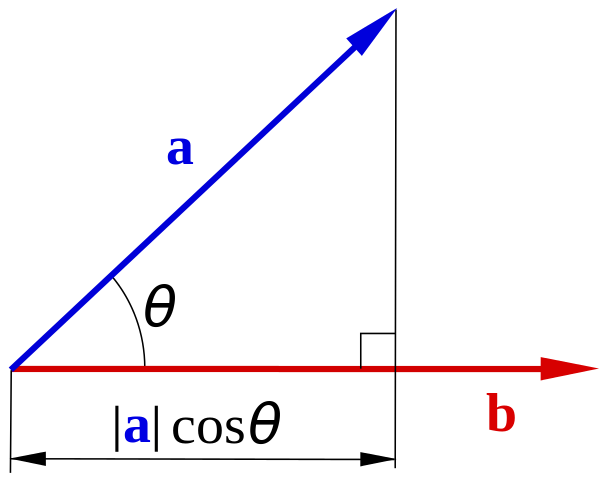
\includegraphics[width=0.8\textwidth]{605px-Scalar-product-dot-product.svg.png}
            \caption{Scalar Product}
        \end{figure}
    \end{frame}

    \begin{frame}
        \frametitle{Conclusiones}
        \begin{itemize}
            \item En conclusión, el software de búsqueda de palabras clave ha demostrado ser una herramienta altamente beneficiosa para la extracción de información relevante en archivos de texto, y su implementación promete mejorar la eficiencia y productividad en el manejo de grandes volúmenes de datos de texto.
            \item Tras realizar un exhaustivo análisis y evaluación del software de búsqueda de palabras clave en archivos de texto, se han obtenido varios hallazgos significativos. En general, el software demostró ser una herramienta efectiva para identificar palabras clave y términos relevantes en los documentos analizados. Sus algoritmos de búsqueda y filtrado mostraron resultados precisos y presentaron las ocurrencias de palabras clave de manera clara y concisa.
        \end{itemize}
    \end{frame}
    
\end{document}